\documentclass[12pt,a4paper]{article}
\usepackage[utf8]{inputenc}
\usepackage[norsk]{babel}
\usepackage{amsmath, amssymb, amsthm}  % For mathematical notation
\usepackage{algorithm, algorithmic}    % For writing algorithms
\usepackage{enumitem}
\usepackage{booktabs}
\usepackage{graphicx}                  % For including images
\usepackage{hyperref}                  % For hyperlinks
\usepackage{pgfplots}                  % For graphs
\pgfplotsset{compat=1.16}
\hypersetup{
    colorlinks=false,
    pdfborder={0 0 0},
}

\title{Øving 9 - Algoritmer og datastrukturer}
\author{Henrik Halvorsen Kvamme}
\date{\today}

\begin{document}

\begin{center}
    
\includegraphics[width=0.5\textwidth]{../images/NTNU_Logo.png}
    
    \vspace{1.5em}  % Optional vertical space
    
    {\LARGE \textbf{Øving 9} \\[0.5em] \text{Algoritmer og Datastrukturer}}  % Title
    \vspace{1em}  % Optional vertical space
    
    {\large Henrik Halvorsen Kvamme}\\  % Author name
    \vspace{0.5em}  % Optional vertical space
    
    {\today}  % Date
\end{center}

\vspace{2em}

\tableofcontents

\newpage

\section{Introduksjon}
Denne rapporten beskriver utviklingen av et program for å finne den korteste veien mellom to punkter ved hjelp av Dijkstras algoritme. Formålet er å demonstrere anvendelsen av denne algoritmen i et veikart for å finne den mest effektive ruten. I tillegg vil rapporten dekke teoretisk grunnlag, implementasjonsdetaljer, og presentasjonen av den grafiske reiseruten.

\section{Teori}
\subsection{Grafteori og Dijkstras algoritme}
En av de grunnleggende algoritmene innen grafteori er Dijkstras algoritme, som finner den korteste veien fra en node til alle andre noder i en vektet graf. Dette er spesielt nyttig for veikart der veier har ulike lengder.

\subsection{Dijkstras algoritme}
Dijkstras algoritme er en greedy algoritme som systematisk velger den veien som ser kortest ut i hvert steg. Algoritmen holder styr på avstanden fra startnoden til hver node og oppdaterer denne avstanden som nødvendig.

\section{Implementasjon}
Programmet er implementert i C++, og bruker en prioritetskø for å holde styr på hvilke noder som skal utforskes. Ved å velge noder med lavest avstand fra startnoden først, sikrer algoritmen at den korteste veien blir funnet på en effektiv måte.

\section{Resultater}
Algoritmen ble testet på et kart over Norden, og resultatene viser at den er i stand til å finne den korteste veien effektivt. Antall noder som algoritmen måtte undersøke, og tidsbruken for forskjellige ruter ble logget.

\begin{figure}[h]
    \centering
    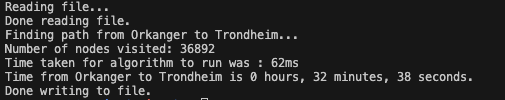
\includegraphics[width=0.8\textwidth]{resultat2.png}
    \caption{Tid fra Orkanger til Trondheim.}
\end{figure}

\begin{figure}[h]
    \centering
    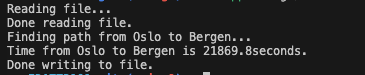
\includegraphics[width=0.8\textwidth]{resultat.png}
    \caption{Tid fra Oslo til Bergen.}
\end{figure}

\section{Kunklusjon}
Dijkstras algoritme viste seg å være et kraftig verktøy for å finne den korteste veien i et stort nettverk av veier. Med en effektiv implementasjon og riktig datastruktur kunne algoritmen raskt prosessere et stort antall noder og finne den mest effektive ruten. Implementasjonen av denne algoritmen demonstrerer potensialet for anvendelse i navigasjonssystemer og ruteplanlegging.

Med mer tid hadde jeg gjerne fullført oppgaven helt.
\end{document}
